%!TEX root = ../rapport.tex

\begin{titlepage}
\newgeometry{top=2cm,bottom=2cm}

\newcommand{\HRule}{\rule{\linewidth}{0.5mm}} % Defines a new command for the horizontal lines, change thickness here

\center % Center everything on the page
 
%----------------------------------------------------------------------------------------
%   HEADING SECTIONS
%----------------------------------------------------------------------------------------


\includegraphics[scale=0.6]{Graphics/LOGO-IPSA.pdf}\\[1.5cm]

\textsc{\Large Projet Electif}\\[0.5cm] % Major heading such as course name
\textsc{\large Projet technique}\\[0.5cm] % Minor heading such as course title

{\normalsize \today}\\[1.5cm]

%----------------------------------------------------------------------------------------
%   TITLE SECTION
%----------------------------------------------------------------------------------------

\HRule \\[0.4cm]
{ \Large \bfseries Evolution de véhicules autonomes dans un environnement urbain intelligent}\\[0.4cm] % Title of your document
\HRule \\[2.5cm]


%----------------------------------------------------------------------------------------
%   LOGO SECTION
%----------------------------------------------------------------------------------------

 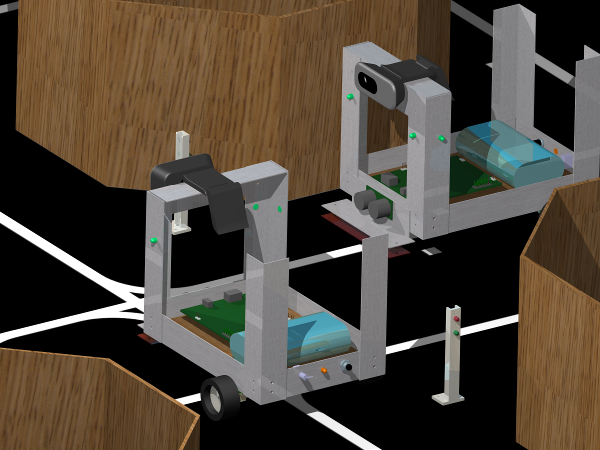
\includegraphics[scale=0.4]{Graphics/illustration2.png}\\[2.5cm]

%----------------------------------------------------------------------------------------
%   AUTHOR SECTION
%----------------------------------------------------------------------------------------
{\normalsize Auteurs:}\\
\small
\textsc{Biton} Guillaume (guillaume.biton@ipsa.fr)\\
\textsc{Guichard} Marc-Antoine \small(marc-antoine.guichard@ipsa.fr)\\
\textsc{Lhermite} Camille \small(camille.lhermite@ipsa.fr)\\
\textsc{Monnot} Maxime \small(maxime.monnot@ipsa.fr)\\[1cm]

 
%----------------------------------------------------------------------------------------

\vfill % Fill the rest of the page with whitespace

\restoregeometry

\end{titlepage}